%==============================================================================
% Sjabloon poster bachproef
%==============================================================================
% Gebaseerd op document class `a0poster' door Gerlinde Kettl en Matthias Weiser
% Aangepast voor gebruik aan HOGENT door Jens Buysse en Bert Van Vreckem

\documentclass[a0,portrait]{hogent-poster}

\usepackage[acronym, toc]{glossaries}
\setglossarystyle{altlist}

\usepackage{float} % Place images where I want

\usepackage{tikz}
\usepackage{pgfplots}
\usepackage{subcaption}

% === Acroniemen ===
\newacronym{auv}{AUV}{Autonomous Underwater Vehicle}
\newacronym{mfls}{MFLS}{Multibeam Forward-Looking Sonar}
\newacronym{cnn}{CNN}{Convolutioneel Neuraal Netwerk}
\newacronym{fcn}{FCN}{Fully Convolutional Network}
\newacronym{rcnn}{R-CNN}{Region-based Convolutional Neural Network}
\newacronym{yolo}{YOLO}{You Only Look Once}
\newacronym{ssd}{SSD}{Single Shot Multibox Detector}
\newacronym{ssl}{SSL}{Semi-Supervised Learning}
\newacronym{self-sl}{Self-SL}{Self-Supervised Learning}
\newacronym{iou}{IoU}{Intersection over Union}
\newacronym{map}{mAP}{Mean Average Precision}
\newacronym{simclr}{SimCLR}{Simple Framework for Contrastive Learning of Visual Representations}
\newacronym{byol}{BYOL}{Bootstrap Your Own Latent}
\newacronym{sss}{SSS}{Side-Scan Sonar}
\newacronym[plural={MILCO's}]{milco}{MILCO}{MIne-Like COntact}
\newacronym[plural={NOMBO's}]{nombo}{NOMBO}{NOn-Mine-like BOttom Object}
\newacronym{dms3}{DMS 3}{Destacamento de Mergulhadores Sapadores}
\newacronym[plural={ROV's}]{rov}{ROV}{Remotely Operated Vehicle}
\newacronym{coco}{COCO}{Common Objects in Context}
\newacronym{uxo}{UXO}{Unexploded Ordnance}
\newacronym{ptu}{PTU}{Pan-Tilt Unit}
\newacronym{dfki}{DFKI}{Deutsches Forschungszentrum für Künstliche Intelligenz}
\newacronym{cas}{CAS}{Continuous Active Sonar}
\newacronym{ar}{AR}{Augmented Reality}
\newacronym[description={\gls{non_max_suppression}}]{nms}{NMS}{Non-Maximum Suppression}
\newacronym{voc}{VOC}{Visual Object Classes}
\newacronym{mse}{MSE}{Mean Squared Error}
\newacronym{kl}{KL}{Kullback-Leibler}
\newacronym{nlp}{NLP}{Natural Language Processing}
\newacronym{vae}{VAE}{Variational Autoencoder}
\newacronym{gan}{GAN}{Generative Adversarial Networks}
\newacronym{nt-xent}{NT-Xent}{Normalized Temperature-scaled Cross Entropy}
\newacronym{moco}{MoCo}{Momentum Contrast}
\newacronym{ema}{EMA}{Exponential Moving Average}
\newacronym{cpu}{CPU}{Central Processing Unit}
\newacronym{gpu}{GPU}{Graphics Processing Unit}
\newacronym{tpu}{TPU}{Tensor Processing Unit}
\newacronym{asic}{ASIC}{Application Specific Integrated Circuit}
\newacronym{fair}{FAIR}{Facebook AI Research}
\newacronym{rpn}{RPN}{Region Proposal Network}
\newacronym{roi}{RoI}{Region of Interest}
\newacronym{amp}{AMP}{Automatic Mixed Precision}

% === Termen ===
\newglossaryentry{blindganger}
{
    name={Blindganger},
    text={blindganger},
    description={Explosief dat niet is afgegaan},
    plural={blindgangers},
    descriptionplural={Explosieven die niet zijn afgegaan.}
}

\newglossaryentry{bounding_box}
{
    name={Bounding box},
    text={bounding box},
    description={Rechthoek om een object op een afbeelding te identificeren en te lokaliseren},
    plural={bounding boxes},
    descriptionplural={Rechthoeken om objecten op een afbeelding te identificeren en te lokaliseren}
}

\newglossaryentry{batch}
{
    name={Batch},
    text={batch},
    description={Groep van samples die gebruikt worden in één trainingsstap. \autocite{Geron_2023}},
    plural={batches},
    descriptionplural={Groepen van samples die gebruikt worden in één trainingsstap. \autocite{Geron_2023}}    
}

\newglossaryentry{batch_size}
{
    name={Batch size},
    text={batch size},
    description={Het aantal samples die gebruikt worden in één trainingsstap. \autocite{Geron_2023}}
}

\newglossaryentry{mini_batch}
{
    name={Mini-batch},
    text={mini-batch},
    description={Kleine, meer behapbare subset van een batch om het geheugengebruik tijdens training te optimaliseren. \autocite{Geron_2023}},
    plural={mini-batches},
    descriptionplural={Kleine, meer behapbare subsets van een batch om het geheugengebruik tijdens training te optimaliseren. \autocite{Geron_2023}}    
}

\newglossaryentry{learning_rate}
{
    name={Learning rate},
    text={learning rate},
    description={Hyperparameter die bepaalt hoe snel het model convergeert richting het minimum van de \gls{loss_functie}. \autocite{Geron_2023}},
}

\newglossaryentry{precision}
{
    name={Precision},
    text={precision},
    description={Een metriek om de accuraatheid van de positieve voorspellingen van het model te meten. Een hoge precision betekent dat het model een lage hoeveelheid \emph{false-positives} voorspelt. Wanneer dit model iets als positief voorspelt, is de kans groot dat dit correct is. 
        $$
        \text{Precision} = \frac{\text{True Positives}}{\text{True Positives} + \text{False Positives}}
        $$
        \autocite{Geron_2023}}
}

\newglossaryentry{recall}
{
    name={Recall},
    text={recall},
    description={Een metriek om te meten hoe goed het model alle relevante positieve datapunten kan voorspellen. Een hoge recall betekent dat het model heel goed is in het correct voorspellen van alle positieve datapunten, zelfs als dit betekent dat het meer \emph{false-positives} voorspelt.
        $$
        \text{Recall} = \frac{\text{True Positives}}{\text{True Positives} + \text{False Negatives}}
        $$
        \autocite{Geron_2023}}
}

\newglossaryentry{portaalkraan}
{
    name={Portaalkraan},
    text={portaalkraan},
    description={Een (meestal verrijdbaar) hijswerktuig, opgebouwd uit een portaal waarop een kraan gemonteerd is die verplaatsbaar is langs de horizontale draagbalk. Meestal wordt deze kraan gebruikt op kaden om o.a. containers uit te laden.}
}

\newglossaryentry{overfitting}
{
    name={Overfitting},
    text={overfitting},
    description={Een fenomeen in machine learning en deep learning waarbij het model de trainingsdata te goed leert -- inclusief ruis en outliers -- in plaats van te generaliseren. Dit zorgt ervoor dat het model excellent presteert op de trainingsdata, maar zeer slecht op ongeziene data.}
}

\newglossaryentry{non_max_suppression}
{
    name={Non-Maximum Supression},
    description={Een techniek in computervisie die wordt gebruikt om overlappende detecties te filteren en alleen de meest waarschijnlijke objectlocaties te behouden. Het selecteert de detectie met de hoogste score en onderdrukt omliggende detecties met een hoge overlap (op basis van de \gls{iou}-score), waardoor dubbele detecties worden verminderd en de nauwkeurigheid van objectdetectie-algoritmes wordt verbeterd. \autocite{Geron_2023}}
}

\newglossaryentry{loss_functie}
{
    name={Loss-functie},
    text={loss-functie},
    description={Wiskundige functie die de afwijking meet tussen de voorspellingen van een model en de werkelijke waarden. Het doel is om deze afwijking te minimaliseren tijdens het trainen van het model, zodat de nauwkeurigheid van de voorspellingen verbetert. Hoe lager de waarde van de loss-functie, hoe beter het model presteert. \autocite{Geron_2023}}
}

\newglossaryentry{thermocline}
{
    name={Thermocline},
    text={thermocline},
    description={De overgang tussen twee lagen water (of lucht) met verschillende temperatuur en dichtheid, in bijvoorbeeld meren of oceanen.},
    plural={thermoclines},
    descriptionplural={De overgangen tussen twee lagen water (of lucht) met verschillende temperatuur en dichtheid, in bijvoorbeeld meren of oceanen.}
}

\newglossaryentry{confidence_score}
{
    name={Confidence score},
    text={confidence score},
    description={De zekerheid van het model dat de voorspelling juist is. \autocite{Geron_2023}},
    plural={confidence scores},
    descriptionplural={De zekerheid van het model dat de voorspellingen juist zijn. \autocite{Geron_2023}}    
}

\newglossaryentry{batch_normalisatie}
{
    name={Batch normalisatie},
    text={batch normalisatie},
    description={Techniek in deep learning die de invoer van elke laag normaliseert (per batch) waardoor de training minder gevoelig wordt voor initiële waarden van de gewichten en \gls{learning_rate}. \autocite{Geron_2023}}
}

\newglossaryentry{backpropagation}
{
    name={Backpropagation},
    text={backpropagation},
    description={Algoritme om parameters in neurale netwerken te updaten en het model zo te trainen. Het werkt door de fout tussen de voorspelde en werkelijke output terug te propageren door het netwerk, waarbij de gradiënt van de fout ten opzichte van de gewichten wordt berekend. Deze informatie wordt vervolgens gebruikt om de gewichten an te passen, zodat het netwerk beter presteert bij toekomstige voorspellingen. \autocite{Geron_2023}}
}

\newglossaryentry{gradient_descent}
{
    name={Gradient descent},
    text={gradient descent},
    description={Wiskundig optimalisatie-algoritme dat stap voor stap het minimum van een functie zoekt door telkens in de richting van de grootste daling (de negatieve gradiënt) te bewegen. Dit algoritme gebruikt de gradiënten van de \gls{loss_functie} die door het \gls{backpropagation}-algoritme berekend zijn om de daadwerkelijke parameters aan te passen, zodat de fout afneemt. \autocite{Geron_2023}}
}

\newglossaryentry{buffer_underflow}
{
    name={Buffer underflow},
    text={buffer underflow},
    description={Numerieke fout die ontstaat wanneer een getal (bv. een gradiënt) zo klein is dat het niet nauwkeurig kan worden opgeslagen in \texttt{float16}-formaat en dus afgerond wordt naar nul. Dit heeft als gevolg een verlies van precisie en een slecht of instabiel leerproces. \autocite{Micikevicius_2017}}
}
\graphicspath{{../graphics/}}

% Info over de opleiding
\course{Bachelorproef}
\studyprogramme{toegepaste informatica}
\academicyear{2024-2025}
\institution{Hogeschool Gent, Valentin Vaerwyckweg 1, 9000 Gent}

% Info over de bachelorproef
\title{Objectdetectie in sonardata met behulp van semi- en self-supervised learning}
\subtitle{Een verkennend onderzoek naar het toepassen van moderne leertechnieken op onderwaterbeeldvorming}
\author{Yoran Gyselen}
\email{yoran.gyselen@student.hogent.be}
\supervisor{Chantal Teerlinck}
\cosupervisor{Stefanie Duyck (Exail Robotics Belgium)}

% Indien ingevuld, wordt deze informatie toegevoegd aan het einde van de
% abstract. Zet in commentaar als je dit niet wilt.
\specialisation{AI \& Data Engineering}
\keywords{Objectdetectie, Semi-supervised, Self-supervised, Sonar-data}
\projectrepo{https://github.com/YoranGyselen-Hogent/bap-2425-yorangyselen}

\begin{document}

\maketitle

\begin{abstract}
Het trainen van deep learning-modellen voor objectdetectie vereist doorgaans grote hoeveelheden gelabelde data. In domeinen zoals sonarbeeldvorming, waar dergelijke data schaars en moeilijk te annoteren is, vormt dit een aanzienlijke belemmering. Dit onderzoek onderzoekt hoe semi-supervised en self-supervised leermethoden deze afhankelijkheid kunnen verminderen, met behoud van nauwkeurigheid. Er worden drie benaderingen vergeleken: een volledig supervised model (Faster R-CNN), een semi-supervised model (FixMatch), en een self-supervised aanpak waarbij BYOL-pretraining wordt gebruikt als feature-extractor in Faster R-CNN. Alle modellen zijn geëvalueerd op een publieke dataset met 7600 gelabelde sonarbeelden. Bij het supervised model daalt de nauwkeurigheid aanzienlijk bij minder gelabelde data, met mAP-scores van 0.7717 (100\%) tot 0.2799 (1\%). FixMatch toont duidelijk betere prestaties bij beperkte labels: mAP van 0.6649 bij 5\% en 0.6828 bij 10\% gelabelde data. De beste prestaties bij lage annotatieniveaus worden echter behaald met self-supervised pretraining: BYOL in combinatie met Faster R-CNN behaalt mAP-scores van 0.6452 (5\%) en 0.7230 (10\%). De resultaten tonen aan dat zowel semi- als self-supervised methoden effectief het aantal benodigde labels kunnen verlagen. Vooral self-supervised pretraining blijkt waardevol in dataschaarse scenario’s. Deze bevindingen bieden perspectief voor efficiëntere workflows in sonarbeeldanalyse en vergelijkbare domeinen waar gelabelde data beperkt beschikbaar zijn.
\end{abstract}

\begin{multicols}{2} % This is how many columns your poster will be broken into, a portrait poster is generally split into 2 columns

\section{Introductie}

In moderne AI-toepassingen, en met name in complexe taken zoals objectdetectie, vormt het verzamelen en annoteren van voldoende gelabelde data vaak een grote uitdaging. Dit is zeker het geval binnen de context van sonarbeeldvorming, waar gelabelde datasets zeldzaam zijn en handmatige annotatie bijzonder arbeidsintensief en kostbaar is. Dit onderzoek vertrekt vanuit de centrale vraag hoe SSL en Self-SL technieken het labelproces kunnen versnellen zonder significante afbreuk te doen aan de nauwkeurigheid van objectdetectiemodellen. Door het inzetten van methodes die leren van grotendeels ongelabelde data, biedt dit onderzoek mogelijke oplossingen voor data-schaarsere omgevingen zoals sonarbeeldanalyse.

\section{Experimenten}

Om de onderzoeksvraag te beantwoorden, werden drie benaderingen experimenteel getest op een publieke dataset van 7600 sonarbeelden: een volledig gesuperviseerd model (Faster R-CNN), een SSL-methode (FixMatch), en een Self-SL-strategie waarbij een BYOL-model eerst werd gepretraind zonder labels. De resultaten tonen aan dat het gesuperviseerde model hoge nauwkeurigheid behaalde bij 100\% gelabelde data, maar sterk in performance daalde bij minder beschikbare labels. FixMatch wist bij 5\% en 10\% gelabelde data merkbaar betere prestaties neer te zetten dan het baseline-model, door slim gebruik te maken van pseudo-labeling en consistency training. De best presterende aanpak was echter Self-SL pretraining met BYOL, waarbij de gegenereerde representaties als backbone dienden voor een Faster R-CNN model. Deze strategie benaderde bij slechts 10\% gelabelde data bijna het prestatieniveau van volledige supervisie. Dit bevestigt het potentieel van Self-SL representatieleren als krachtige methode in situaties met beperkte annotatiecapaciteit.

\begin{figure}[H]
    \centering
    \begin{subfigure}{.2\linewidth}
        \centering
        \captionsetup{justification=centering}
        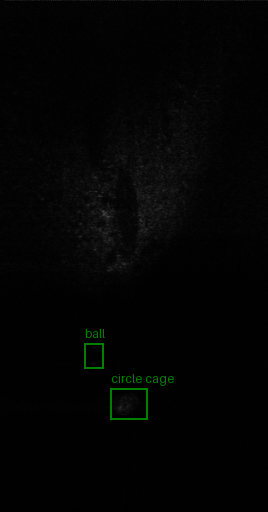
\includegraphics[width=0.9\linewidth]{1_gt.png}
        \caption{Ground truth}
    \end{subfigure}%
    \hfill
    \begin{subfigure}{.2\linewidth}
        \centering
        \captionsetup{justification=centering}
        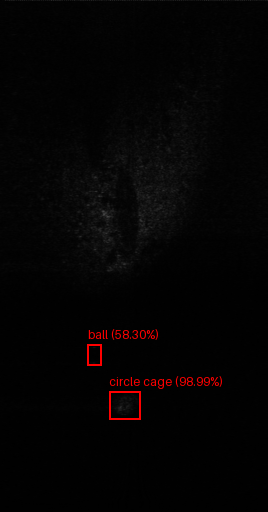
\includegraphics[width=0.9\linewidth]{1_fixmatch_10pct.png}
        \caption{FixMatch 10\%}
    \end{subfigure}%
    \hfill
    \begin{subfigure}{.2\linewidth}
        \centering
        \captionsetup{justification=centering}
        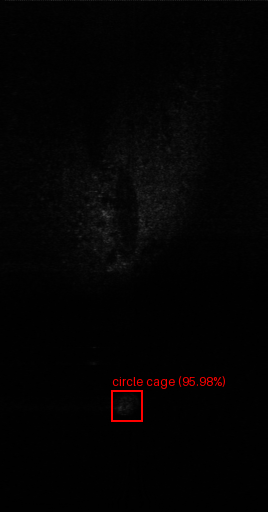
\includegraphics[width=0.9\linewidth]{1_fixmatch_5pct.png}
        \caption{FixMatch 5\%}
    \end{subfigure}%
    \hfill
    \begin{subfigure}{.2\linewidth}
        \centering
        \captionsetup{justification=centering}
        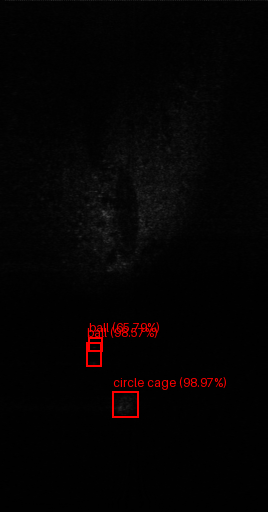
\includegraphics[width=0.9\linewidth]{1_faster_rcnn_10_byol.png}
        \caption{BYOL 10\%}
    \end{subfigure}%
    \hfill
    \begin{subfigure}{.2\linewidth}
        \centering
        \captionsetup{justification=centering}
        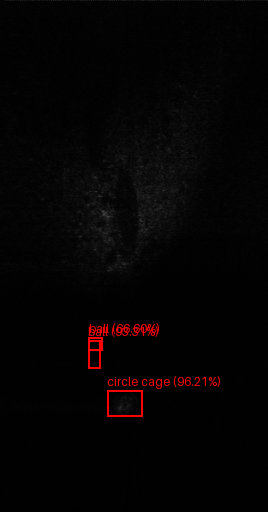
\includegraphics[width=0.9\linewidth]{1_faster_rcnn_5_byol.png}
        \caption{BYOL 5\%}
    \end{subfigure}%
    \caption{Voorspellingen op afbeelding \texttt{00001} van de \texttt{UATD\_Test\_1}-dataset door FixMatch en Faster R-CNN + BYOL getraind op verschillende subsets.}
\end{figure}

\section{Conclusies}

De experimenten tonen aan dat zowel SSL als Self-SL effectieve strategieën zijn om de afhankelijkheid van gelabelde data bij objectdetectie in sonarbeelden te verminderen. Terwijl het volledig gesuperviseerde Faster R-CNN-model hoge prestaties behaalde bij volledige annotatie, daalde de nauwkeurigheid sterk bij minder gelabelde data. SSL met FixMatch bood hierbij een aanzienlijke verbetering door effectief gebruik te maken van ongelabelde data via pseudo-labeling, vooral bij 5\% en 10\% gelabelde data. De beste resultaten werden echter bereikt met Self-SL via BYOL, waarbij pretraining op ongesuperviseerde beelden leidde tot robuuste representaties die, eenmaal geïntegreerd in een Faster R-CNN, bijna het prestatieniveau van het volledig gesuperviseerde model evenaarden bij slechts 10\% gelabelde data. Hiermee bevestigen de resultaten dat FixMatch en vooral BYOL veelbelovende technieken zijn voor objectdetectie in data-schaarsere contexten zoals sonarbeeldanalyse.

\begin{figure}[H]
    \centering
    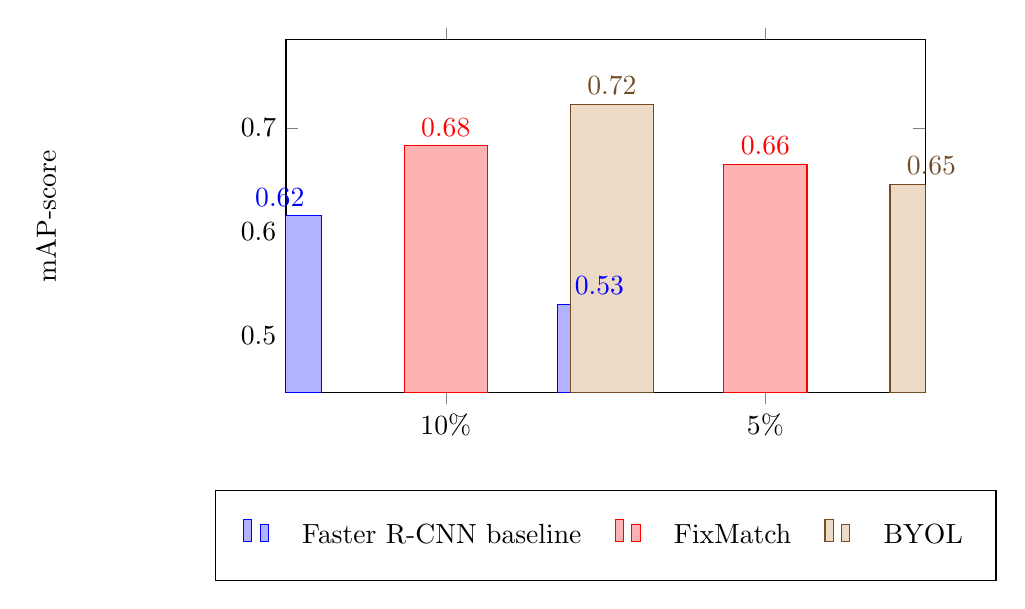
\begin{tikzpicture}
        \begin{axis}[
            ybar,
            bar width=30pt,
            width=0.8\linewidth,
            height=0.5\linewidth,
            enlargelimits=0.5,
            ybar=30pt,
            legend style={
                at={(0.5,-0.20)},
                anchor=north,
                legend columns=-1,
                inner sep=10pt,
                outer sep=10pt,
                row sep=5pt,
                column sep=10pt,
            },
            xlabel={Verschillende data-splits},
            xlabel style={yshift=-20pt},
            ylabel={mAP-score},
            ylabel style={yshift=60pt},
            ymax=0.7,
            symbolic x coords={10\%, 5\%},
            xtick=data,
            nodes near coords,
            nodes near coords align={vertical},
            ]
            \addplot coordinates {(10\%,0.6152) (5\%,0.5298)};
            \addplot coordinates {(10\%,0.6828) (5\%,0.6649)};
            \addplot coordinates {(10\%,0.7230) (5\%,0.6452)};
            \legend{Faster R-CNN baseline, FixMatch, BYOL}
        \end{axis}
    \end{tikzpicture}
    \caption{Overzicht van de mAP voor het supervised Faster R-CNN model, het SSL FixMatch model en het Self-SL BYOL model, getraind op 10\% en 5\% data-splits.}
\end{figure}

\section{Toekomstig onderzoek}

Hoewel dit onderzoek de meerwaarde van zowel SSL als Self-SL bij objectdetectie op sonarbeelden aantoont, blijven er diverse beloftevolle onderzoekspistes open. Zo is het waardevol om alternatieve Self-SL pretrainingsmethoden zoals SimCLR, MoCo of DINO te vergelijken met BYOL, evenals verschillende backbone-architecturen zoals Swin Transformer of ConvNeXt te evalueren op hun geschiktheid voor sonarbeeldvorming. Ook binnen SSL kunnen recente methoden zoals FlexMatch, SoftMatch of UDA, in combinatie met domeinspecifieke augmentaties, mogelijk betere prestaties leveren dan FixMatch. Een veelbelovende richting is het combineren van Self-SL pretraining met SSL fine-tuning om de voordelen van beide benaderingen te benutten. Verder kan transfer learning op basis van grootschalige, ruwe sonardata bijdragen aan de ontwikkeling van generieke sonarbackbones voor uiteenlopende toepassingen. Tot slot kan onderzoek naar actieve labelselectie en foutenanalyse helpen om annotatie-efficiëntie te verhogen en modelbetrouwbaarheid te verbeteren in kritieke contexten zoals defensie of onderwaterrobotica.

\end{multicols}
\end{document}